\section{Lineare Gleichungssysteme}\index{Gleichungssysteme}\index{lineare Gleichungssysteme}

\subsection*{Lernziele}
\begin{itemize}
	\item{Lineare Gleichung mit mehreren unbekannten}
	\item{Grundform}
	\item{Lösungsmethoden}
	\begin{itemize}
		\item{Einsetzungsverfahren}
		\item{Additionsverfahren}
		\item{Graphische Methode}
		\item{Taschenrechner}
      \TALS{\item 3x3 Gleichungssysteme}
		\item{Substitution}
      \TALS{\item Gleichungssysteme mit Parametern und Fallunterscheidung}
    \item Textaufgaben
	\end{itemize}

\end{itemize}

%%\TALSTadBFWA{124}{2.5.1}
\TadBMTA{135}{9}
\newpage

\subsection{Einstiegsbeispiel}
Ein Apfel koste CHF $a$, eine Banane CHF $b$. Wenn ich drei Äpfel und zwei Bananen kaufe, bezahle ich CHF 3.10. Wenn ich hingegen vier Äpfel und fünf Bananen kaufe, so muss ich CHF 6.00 bezahlen. Wie viel kostet ein Apfel, wie viel eine Banane?

\begin{center}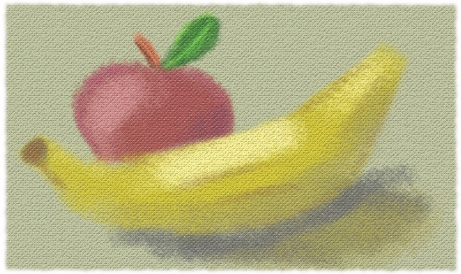
\includegraphics[width=8cm]{allg/gls/img/ApfelBanane.jpg}\end{center}

\TNT{8}{$a$ = Preis eines Apfels \textbf{in} CHF

  $b$ = Preis einer Banane \textbf{in} CHF

  $3a$ = Totalpreis von drei Äpfeln \textbf{in} CHF

  $2b$ = Totalpreis von zwei Bananen \textbf{in} CHF

  $3a+2b$ = Totalpreis von drei Äpfeln und zwei Bananen \textbf{in} CHF
  
  \vspace{22mm}
}

Diese Term-Information packen wir in Gleichungen und schreiben die
beiden Gleichungen als sortiertes \textit{(lineares)} Gleichungssystem auf:

\TNTeop{\gleichungZZ{3a + 2b}{3.10}{4a + 5b}{6.00}}

%%%%%%%%%%%%%%%%%%%%%%%%%%%%%%%%%%%%%%%%%%%%%%%%%%%%%%%%%%%%%%%%%%%%%%%%%%

\subsection{Einsetzungsverfahren}\label{einsetzungsverfahren}\index{Einsetzungsverfahren!Gleichungssysteme}
Beim Einsetzungsverfahren wird aus einer der beiden Gleichungen eine der beiden Variablen alleine gestellt. Zum Beispiel hier aus der zweiten Gleichung $b = ...$; danach wird dieser $b$-Term in die \textbf{andere} Gleichung eingesetzt, und so erhalten wir eine Gleichung mit einer Unbekannten.



\gleichungsSystemNummeriert{3a+2b}{3.10}{4a+5b}{6.00}

%%\gleichungZZ{3a + 2b}{3.10\TRAINER{ (I)}}{4a + 5b}{6.00\TRAINER{ (II)}}

1. Aus der zweiten Gleichung erhalten wir für $b$:

\TNT{3.2}{$$5b= 6 - 4a \Longrightarrow b = {\color{orange}\frac{6.00-4a}{5}}. (III)$$}

2. Diesen Term setzen wir nun für $b$ in die \textbf{andere} (hier die obere) Gleichung ein:
$$3a+2b = 3.10$$

Dies ergibt für $a$:

\TNT{1.2}{$$3a+2\cdot{}{\color{orange}\frac{6.00 - 4a}{5}} = 3.10.$$}

3. Wenn wir diese Gleichung nun nach $a$ auf"|lösen, ...

\TNT{4}{
  $$ 3a+\frac{12-8a}{5} = 3.1$$
  $$ 3a+\frac{12}{5} - \frac{8a}{5} = 3.1$$
  $$ 15a+12 - 8a = 15.50$$
  $$ 7a = 3.50$$
}

so erhalten wir $a = \LoesungsRaum{0.50}$ (CHF).


4. Nun setzen wir das gefundene $a$ in (III) ein:

\TNT{2}{$b=\frac{6-4a}{5} = \frac{6-4\cdot{} 0.5}{5} = \frac{6-2}{5} =
  \frac{4}{5} = 0.8$}%% end TNT

...und erhalten $b = \LoesungsRaum{0.80}$ (CHF).


\newpage

  \begin{gesetz}{Lösungsmenge}{}
    Die Lösung eines Gleichungssystems ist typischerweise ein
    geordnetes Zahlenpaar. Wir schreiben 

\TNT{2}{    $$\LoesungsMenge{}_{(a; b)} = \left\{(0.50; 0.80)\right\}$$ } 

  als Beispiel für obige Gleichung.
    
    \end{gesetz}


  \begin{rezept}{Einsetzungsverfahren}{}
  \begin{enumerate}

  \item Eine (beliebige) Gleichung nach einer (beliebigen) Variable
    auf\/lösen (separieren), falls nicht schon geschehen
  \item Den Term (Wert) der Variable in die \textbf{andere(n)}
    Gleichung(en) einsetzen
  \item Die neue(n) Gleichung(en) wie gewohnt auf\/lösen
  \item Das Resultat in die Gleichung aus Schritt 1 einsetzen,
    um die dortige Variable zu erhalten
  \end{enumerate}
\end{rezept}


\subsection*{Aufgaben}
%%  \AadBMTA{151}{8. d) h) und 9. a)}
\GESO{\olatLinkArbeitsblatt{Gleichungssysteme}{https://olat.bms-w.ch/auth/RepositoryEntry/6029794/CourseNode/112603866030292}{Kap. 1: a) b) c) g) h)}}
\TALS{\olatLinkArbeitsblatt{Gleichungssysteme}{https://olat.bms-w.ch/auth/RepositoryEntry/6029786/CourseNode/112603866140343}{Kap. 1: a) b) c) g) h)}}
\newpage
  
\subsubsection{Ein nicht lineares Beispiel (optional)}
Mit dem Einsetzungsverfahren lassen sich auch nicht-lineare
Gleichungssysteme lösen:
\gleichungZZ{a\cdot{}b}{72}{a^4\cdot{}\frac{b}2}{288}

Lösungsweg:
  \TNT{10.8}{
    Erstens aus der ersten Gleichung das $b$ separieren:
    $$b = \frac{72}a \hspace{40mm} (I)$$
    Und dieses $b$ nun in die \textbf{andere} Gleichung einsetzen:
    $$a^4\cdot{}\frac12\cdot{}\frac{72}{a} = 288$$
    
    Auf\/lösen nach $a$:

    $$a^3 \cdot{} 36 = 288$$

    $$a^3 = 8$$

    ergibt $a=2$.

    Dies nun in die «separierte
    Gleichung» $(I)$ einsetzen: $b=\frac{72}{a} = \frac{72}2 = 36$.

    Hinweis: Hier hätte man gleich von vornherein die zweite Gleichung
    durch die erste dividieren können (dies wäre dann aber nicht mehr
    das Einsetzungsverfahren).
  }%%

\newpage
%%%%%%%%%%%

\subsection{Additions- bzw. Subtraktionsverfahren}\index{Additionsverfahren!lineare Gleichungen}\index{Subtraktionsverfahren!Gleichungssysteme}
Eine weitere Möglichkeit lineare Gleichungssysteme mit mehreren Unbekannten zu lösen ist das Verfahren, die linke und die rechte Seite miteinander zu addieren (bzw. voneinander zu subtrahieren), sodass eine Variable wegfällt. Dazu müssen die Gleichungen vorher so \textit{präpariert} werden, dass in einer Variablen (hier \zB $x$) die Koeffizienten übereinstimmen:

\gleichungsSystemNummeriert{6x+7y}{3}{8x-2y}{38}
%%\gleichungZZ{4x+4y}{48\hspace{10mm}\text{ (I)}}{3x-6y}{-27\hspace{5mm}\text{ (II) }}

Wir wählen \zB in obigem Beispiel die Variable $x$ und suche zunächst
das kleinste gemeinsame Vielfache 24. Nun multiplizieren wir die obere
Gleichung mit 4 und die untere mit 3 und erhalten:


%%\TNT{2.8}{\gleichungZZ{12x+12y}{144 \hspace{8mm}(I)}{12x-24y}{-108\hspace{5mm} (II)}}
\TNT{2.8}{\gleichungsSystemNummeriert{24x+28y}{12}{24x-6y}{114}}


Nun können wir die untere Gleichung (II) von der oberen Gleichung (I) abziehen (damit die Variable $x$ eliminiert wird)
und erhalten:
  
\TNT{3.2}{
 (I) - (II)
  $$(24x+28y)  - (24x-6y)  = 12 - 114$$
  $$24x+28y  - 24x+6y  = -102$$
  $$0x + 34y = -102$$
  $$y=-3$$
}


  Dieses $y$ setzen wir \zB in die Gleichung $8x-2y=38$ ein:
  \TNTeop{
    $$8x -2 \cdot{}(-3) = 38 \hspace{5mm}| TU$$
    $$8x +6 = 38 \hspace{5mm}| -6$$
    $$8x  = 32 \hspace{5mm}| :8$$
    $$x = 4$$

    $$\mathbb{L}_{(x;y)} = \left\{ (4; -3)  \right\}$$
}
\newpage


  \begin{rezept}{Rechengesetz Additionsverfahren}{gesetz_additionsverfahren}
    Eine beliebige Variable wird gewählt und danach beide Gleichungen so multipliziert,
    dass die Zahlen vor dieser Variable in beiden Gleichungen gleich werden.

    Dies funktioniert
    immer mit einem gemeinsamen Vielfachen der beiden Zahlen.
  \end{rezept}

\subsection*{Aufgaben}
\AadBMTA{150}{7. g) b) c) e)}

\newpage

  
\subsection{Graphische Methode}\index{graphische Methode!Gleichungssysteme}

\subsubsection{Gleichsetzungsverfahren (optional)}\label{lin_gl_gleichsetzungsverfahren}\index{Gleichsetzungsverfahren}
Beim Gleichsetzungsverfahren werden zwei Gleichungen nach der selben Variable \textit{aufgelöst} und die beiden Gleichungen der Form $a = ...$ einander gleichgesetzt.

\gleichungZZ{a}{{\color{orange}\frac{3.10 -  2b}{3}}}{a}{{\color{ForestGreen}\frac{6.00 - 5b}{4}}}%%
\vspace{22mm}

Setzen wir nun die beiden Terme gleich, so erhalten wir die
folgende Gleichung:

\TNT{7.2}{$${\color{orange}\frac{3.10 - 2b}{3}} =
  {\color{ForestGreen}\frac{6.00 - 5b}{4}}$$
  \vspace{10mm}

  Links mit 4, rechts mit 3 erweitern
  $$4\cdot{}(3.10-2b) = 3\cdot{}(6.00-5b)$$
  $$12.40 - 8b = 18 - 15b$$
  $$7b = 5.60$$
  
}%% END TNT

%%Nach Auf"|lösung erhalten wir $b=\LoesungsRaum{0.80}$ (CHF) und das $a$ erhalten wir danach durch Einsetzen in eine der beiden bereits nach $a$ aufgelösten Gleichungen: $a=\LoesungsRaum{0.50}$ (CHF).
Nach Auf"|lösung erhalten wir $b=\LoesungsRaum{0.80}$ (CHF) und das
$a$ erhalten wir danach durch Einsetzen in eine der beiden bereits
nach $a$ aufgelösten Gleichungen:

\TNT{4}{
$$a=\frac{3.10 -2b}{3} =\frac{3.10 - 2\cdot{}0.80}{3} =  \frac{3.10 -
    1.60}{3} =  \frac{1.50}{3} = 0.50 $$
}
Das Gleichsetzungsverfahren ist ein Spezialfall des
Einsetzungsverfahrens\totalref{einsetzungsverfahren}.
\newpage



%%%%%%%%%%%%%%%%%%%%%%%%%%%%%%%%%%%%%%%%%%%%%%%%%%%%%%%%%%%%%%%%%%%%%%%%%%%%%%%%%%%%%

\subsubsection{Ablesen}
Das Gleichsetzungsverfahren\totalref{lin_gl_gleichsetzungsverfahren} kann auch als Schnittpunkt zweier linearer Funktionen\totalref{lineare_funktionen}
aufgefasst werden. Betrachten wir folgende beiden Gleichungen:

\gleichungZZ{2x - 10y}{-10}{6x+15y}{60}

Lösen wir beide Gleichungen nach $y$ auf, so erhalten wir zwei Funktionsgleichungen:

\gleichungZZ{f: y}{\noTRAINER{...............}\TRAINER{0.2x + 1}}{g:y}{\noTRAINER{...............}\TRAINER{-\frac{2}{5}x + 4}}


Zeichnen Sie die beiden linearen Funktionen als Graph ins folgende
Koordinatensystem ein und lesen Sie die Lösung \TRAINER{bei $(5|2)$} ab:

\noTRAINER{
  \bbwGraph{-6}{8}{-1}{6}{}
}
\TRAINER{
  \bbwGraph{-6}{8}{-1}{6}{
    \bbwFuncC{\x * 0.2 + 1}{-5.5:8}{green}
    \bbwLetter{7.5,3}{f}{green}
    \bbwFuncC{-0.4*\x + 4}{-1:7}{blue}
    \bbwLetter{7.5,1}{g}{blue}
  }
}
\newpage


\subsection*{Aufgabe Graphisch}
  Lösen Sie die folgende Aufgabe graphisch. Bringen Sie die beiden Gleichungen erst in die Form $y=ax+b$ der linearen Funktionen. Zeichnen Sie danach beide Funktionen in ein Koordinatensystem ($x$ von -6 bis 1 und $y$ von -3 bis 5). Schätzen Sie die Lösung, bevor Sie diese berechnen.
\AadBMTA{151}{8. g)}


\olatLinkGESOKompendium{2.2.4.}{15}{39. bis 41.}

\newpage


\subsection{Lineare Abhängigkeit}\index{abhängig!linear}\index{Lineare
  Abhängigkeit}

Lösen Sie das folgende Gleichungssystem vorerst mit dem
Taschenrechner:

\gleichungZZ{9x-6y}{18}{30x-20y}{60}

Die Lösung ist nicht vielsagend.

Durch die Additionsmethode erhalten wir folgendes Gleichungssystem:

\TNT{3.2}{\gleichungZZ{90x-60y}{180}{90x-60y}{180}}

oder nach der Subtraktion:

\TNT{2}{$$0=0.$$}

Dies bedeutet, wir haben durch Äquivalenzumformungen nun zweimal die selbe
Gleichung da stehen. Wir können $x$ nur in Abhängigkeit von $y$
berechnen (mehr nicht):

$$x=\noTRAINER{\hspace{20mm}}\TRAINER{\frac{6+2y}{3}}$$

Oder wir können $y$ in Abhängigkeit von $x$ berechnen:
$$y=\noTRAINER{\hspace{20mm}}\TRAINER{\frac{3x-6}{2}}$$

Wichtig ist vor allem, dass Sie auch die Antwort des Taschenrechners verstehen!


%
% Spezialfälle linearer Gleichungssysteme (leere menge/unendlich viele Lösungen)
%
\subsubsection{Spezialfälle}
\textbf{TYP A:} Keine Lösung

Bestimmen Sie die Lösungsmenge des folgenden linearen Gleichungssystems:

\gleichungZZ{2x-y}{1}{4x-2y}{3}           

\TNT{2}{Additionsverfahren liefert $$(4x-2y)-2\cdot{}(2x-y) = 3 - 2\cdot{}(1) \Longrightarrow 0 = 1$$}

Die Gleichung hat keine Lösung. Geometrisch: Die Geraden sind parallel.

$$\LoesungsMenge{}_{(x;y)} = \LoesungsRaumLang{\{\}}$$

\textbf{TYP B:} Beliebig viele Lösungen (lineare Abhängigkeit)

Bestimmen Sie die Lösungsmenge des folgenden linearen Gleichungssystems:

\gleichungZZ{2x-y}{1}{4x-2y}{2}           

\TNT{2}{Additionsverfahren liefert $$(4x-2y)-2\cdot{}(2x-y) = 2 - 2\cdot{}(1) \Longrightarrow 0 = 0$$}

Hier gibt es unendlich viele Lösungen. Die entsprechenden Geraden sind zusammefallend.

$$\LoesungsMenge{}_{(x;y)} = \LoesungsRaumLen{50mm}{ \left\{(x;y) \text{ mit } y = 2x-1 \Longleftrightarrow x = \frac{y+1}2 \right\} }$$

%%\TRAINER{$y = \frac{9x-4.2}{4.8}$ ist die Funktionsgleichung beider Geraden.}
\newpage

\subsection*{Repetition: Lösungsmenge}\index{Lösungsmenge}
Auch graphisch kann die Lösungsmenge ermittelt werden. Die Angaben
sind ananolg zu den Gleichungen mit einer Variable.
\begin{center}
\begin{tabular}{c|c|c}
schneidend                 & parallel      &
zusammenfallend\\
 & & \\
\vspace{0.5mm}
$\gleichungZZ{y}{x}{y}{8}$ & $\gleichungZZ{y}{x+5}{y}{x+7}$ & $\gleichungZZ{y}{x+3}{2y}{2x+6}$   \\
 & & \\
$\times$                   & //            &   \textbf{/}      \\
 & & \\
$x=8$                      & $5=7$         &  $3=3$            \\
 & & \\
$\lx=\LoesungsRaumLen{20mm}{\{8\}}$                & $\lx=\LoesungsRaumLen{20mm}{\{\}}$    &  $\lx=\LoesungsRaumLen{20mm}{\mathbb{R}}$ \\
\end{tabular} 
\end{center}

%%%%%%%%%%%%%%%%%%%%%%%%%%%%%%%
%\subsection*{Aufgaben}
%%\TALSAadBMTA{125ff}{382. 383., 389. a) 410. a), 411. a) b)}
%\GESO{\olatLinkArbeitsblatt{Gleichungssysteme}{https://olat.bms-w.ch/auth/RepositoryEntry/6029794/CourseNode/112603866030292}{Kap. 1: a) b) c) g) h)}}
%\TALS{\olatLinkArbeitsblatt{Gleichungssysteme}{https://olat.bms-w.ch/auth/RepositoryEntry/6029786/CourseNode/112603866140343}{Kap. 1: a) b) c) g) h)}}
%\AadBMTA{153ff}{Falls nötig zuerst in Grundform bringen. Schreiben Sie $x$, $y$ und $z$ streng untereinander. Danach mit Taschenrechner lösen: 18. a) b) c) und e)}

%Optionale Aufgaben zu linearen Funktionen mit Taschenrechner:
%\AadBMTA{253}{24. b) c) d)  25. a)}

\newpage


\subsection{Taschenrechner}\index{Taschenrechner!Gleichungssysteme}
Lineare Gleichungssysteme sind so zentral, dass viele heutige
Taschenrechner diese lösen kann. Hier nochmals Äpfel und Bananen:

\gleichungZZ{3a + 2b}{3.10}{4a + 5b}{6.00}

\GESO{Suchen Sie \tiprobutton{2nd}\tiprobutton{tan_sys-solv} und geben Sie die Zahlen 3, 2, 3.10, 4, 5 bzw. 6.00 in die entsprechenden Felder ein.}
\TALS{Definieren Sie das Gleichungssystem gls:=\{3a+2b=3.1, 4a+5b=6.0\}. Dies können Sie nun einfach mit solve(gls,\{a, b\}) auflösen lassen.}

\GESO{
\begin{bemerkung}{}{}
  Die Variable beim TI-30 PRO müssen bei 2x2-Gleichungssystemen $x$ und $y$  heißen.
\end{bemerkung}
}

\GESO{
  \subsubsection{Eingabe negativer Zahlen}
  Lösen Sie das folgende Gleichungssystem mit dem Taschenrechner.

  \gleichungZZ{-4x + (-8)y}{16}{3x-5y}{32}

  Beachten Sie die Eingabe negativer Zahlen auf dem TI 30 Pro
  MathPrint. Das negative Vorzeichen wird mit \tiprobutton{neg} eingegeben,
  wohingegen die Subtraktion mit dem einfachen \tiprobutton{minus} eingegeben wird.

  \TNT{2.4}{Lösung: $x=4$, $y=-4$\vspace{22mm}}

}

\GESO{
\aufgabenFarbe{  
  Prüfen Sie mit diesem Wissen von Seite 150ff die Resultate von Aufgabe 7. g) [$x=\frac{42}{61}$ und $y=\frac{60}{61}$], 7. b) [$x=\frac52$ und $y=-\frac{15}{2}$] 8. a) [$x=2$ und $y=6$] und 8. b) [$x=-2$ und $y=2$]
}}

\olatLinkGESOKompendium{2.2.1}{13}{27. bis 30.}
\newpage


%\TALS{\subsection{Drei Unbekannte}\index{Drei unbekannte!Gleichungssysteme}\index{lineare Gleichungssysteme!mit drei Unbekannten}\index{Gleichungssysteme!lineare mit drei Unbekannten}
Das Additionsverfahren funktioniert auch mit mehr als zwei unbekannten. Betrachten wir dazu das folgende lineare Gleichungssystem:

\gleichungDD{2x -3y +4z}{33}{3x+2y-z}{-5}{5x-y-5z}{-12}

Zunächst eliminieren wir die Variable $x$. Dazu erzeugen wir die Gleichung (IV), indem wir die erste Gleichung mit 3 und die zweite Gleichung mit 2 multiplizieren und danach die Gleichungen voneinander abziehen.

(IV)

\TNT{3.6}{\gleichungZZ{6x-9y+12z}{99}{6x + 4y -2z}{-10}
  Daraus ergibt sich (IV):
  $$-13y + 14z = 109$$
}%%

Analog mit Gleichung (II)$\cdot{}5$ und (III)$\cdot{}3$:

(V)

\TNT{3.6}{\gleichungZZ{15x+10y-5z}{-25}{15x-3y-15z}{-36}
  Daraus ergibt sich (V):
  $$13y + 10z = 11$$
}
\newpage
Gleichung (IV) und (V) enthalten nur noch zwei Variable und können nach einem gewohnten Verfahren gelöst werden:

\TNT{12.0}{\gleichungZZ{-13y + 14z}{109}{13y+10z}{11}
  und somit $24z = 120$ und schließlich $z=5$. Dieses $z$ setzen wir in Gleichung (V) ein:
  $$-13y + 10\cdot{}(5) = 11$$
  und wir erhalten $y=-3$

  Zuletzt $z=5$ und $y=-3$ einsetzen in die Gleichung (I):
  $$2\cdot{}x -3\cdot{}(-3) + 4\cdot{}(5) = 33$$
  was uns zu $x=2$ bringt.

  $$\LoesungsMenge{}_{(x;y;z)} = \{(2; -3; 5)\}$$
}%% END TNT

%\newpage}

\TALS{\subsection{3x3-Systeme}

Lösen Sie das folgende 3x3-Gleichungssystem mit dem Taschenrechner:

\gleichungDD{x+2y+3z}{50}{x+z}{16}{2y-z}{7}

\subsection*{Aufgaben}
\AadBMTA{153ff}{21. b) c) e)}
\newpage
}

\subsection{Substitution}\index{Substitution!Gleichungssysteme}\index{Lineare Gleichungssysteme!mit Substitutionsmethode}
Manchmal gibt es Situationen, in denen ein Gleichungssystem besser mit
einer Ersetzung (Substitution) als mit sturem Ausmultiplizieren gelöst
werden kann.

Betrachten Sie einmal das folgende Gleichungssystem:

\gleichungZZ{\frac{2a}{3+b} - \frac{b}{5-a}}{1}{\frac{3a}{b+3} + \frac{2b}{5-a}}{19}

Es ist offensichtlich, dass die Terme $\frac{a}{3+b}$ und
$\frac{b}{5-a}$ mehrfach vorkommen.

Hier bietet sich eine Ersetzung (Substitution) an:

$$X := \LoesungsRaum{\frac{a}{3+b}}$$

und

$$Y := \LoesungsRaum{\frac{b}{5-a}}$$

Das neue entstandene Gleichungssystem ist viel übersichtlicher und
auch einfacher zu lösen:

\TNT{2.4}{\gleichungZZ{2X - Y}{1}{3X+2Y}{19}}

Nach dem Auf"|lösen (\zB Taschenrechner) erhalten wir $X=\LoesungsRaum{3}$ bzw. $Y=\LoesungsRaum{5}$. Mit diesen Werten
können wir $a$ bzw. $b$ bestimmen.
\newpage

\textbf{Rücksubstitution}\index{Rücksubstitution}\,\\

\vspace{1mm}

\TNT{10.8}{

  \gleichungZZ{3}{\frac{a}{3+b}}{5}{\frac{b}{5-a}}

    und somit:

\gleichungZZ{9+3b}{a}{25-5a}{b}

...sortieren...

\gleichungZZ{a-3b}{9}{5a+b}{25}

Nach dem Auf"|lösen erhalten wir:

$$\mathbb{L}_{(a;b)} = \left\{ \left(\frac{21}{4} ;  -\frac{5}{4} \right)  \right\}$$
}%% END TNT


\subsection*{Aufgaben}
\TALSAadBMTA{127ff}{390. b), 391.}
\GESOAadBMTA{152}{12. c), 13. a)}
\olatLinkGESOKompendium{2.2.2}{14}{33. bis 34.}



\subsection{Vermischte Aufgaben}\index{Bruchgleichungen!Gleichungssysteme}
Oft kommen auch in Gleichungssystemen Bruchgleichungen vor. Tipp:
bevor Sie die nachfolgenden Aufgaben lösen, betrachten Sie die folgende
Abkürzung: Um die folgende Bruchgleichung zu vereinfachen...

\gleichungZZ{\frac{\color{ForestGreen}2-x}{\color{red}2x-3}}{\frac{\color{red}5-y}{\color{ForestGreen}2y-4}}{8}{5x-3y}
... wird die erste Gleichung mit «übers Kreuz multiplizieren» zu:

$$({\color{ForestGreen}2-x})({\color{ForestGreen}2y-4}) =
({\color{red}2x-3})({\color{red}5-y})$$
Nun wie gewohnt auflösen:
\TNT{3.2}{
  $$4y-8-2xy+4x=10x-2xy-15+3y$$
  $$\Rightarrow y+7=6x$$
}
Grundform:
\TNT{3.2}{
  \gleichungZZ{6x-y}{7}{5x-3y}{8}
  Additionsverfahren: Obere Gleichung mit 3 multiplizieren:
  \gleichungZZ{18x-3y}{21}{5x-3y}{8}
}%% END TNT

$$\LoesungsMenge{}_{(x;y)} = \LoesungsRaumLang{\{(1; -1)\}}$$


\newpage
\subsection*{Aufgaben}
Lösen Sie die folgenden Aufgaben mit der für Sie am besten geeigneten Methode, indem Sie die
Gleichungen in der Regel zunächst in die Grundform bringen.

%%\TALSAadBMTA{125ff}{382. 383., 389. a) 410. a), 411. a) b)}
\GESO{\olatLinkArbeitsblatt{Gleichungssysteme}{https://olat.bms-w.ch/auth/RepositoryEntry/6029794/CourseNode/112603866030292}{Kap. 9: a) b) c) d) e)}}
\TALS{\olatLinkArbeitsblatt{Gleichungssysteme}{https://olat.bms-w.ch/auth/RepositoryEntry/6029786/CourseNode/112603866140343}{Kap. 9}}
%\AadBMTA{153ff}{Falls nötig zuerst in Grundform bringen. Schreiben Sie $x$, $y$ und $z$ streng untereinander. Danach mit Taschenrechner lösen: 18. a) b) c) 
%\AadBMTA{151}{9. b) d) e) und f)}
%\TALS{  \AadBMTA{158}{58. (Quader) mit Taschenrechner}}

%\olatLinkGESOKompendium{2.2.1}{13}{31. bis 32.}

\newpage


\TALS{\subsection{Gleichungssysteme mit Parametern}\index{Parameter!Gleichungssysteme}\index{Lineare Gleichungssysteme!mit Parametern}
Das folgende Gleichungssystem hat offensichtlich vier und nicht wie
üblich zwei Variable. Wenn wir das System hingegen nach $x$ und $y$
auf"|lösen, so können wir diese beiden Größen
\textbf{in Abhängigkeit} der beiden Parameter\footnote{Parameter =
  Bei- oder Nebenmaß} ($p$ und $q$) ausdrücken.

\gleichungZZ{3x-5y}{p-5q}{5x+6y}{16p+6q}

Zum Lösen können wir wieder mit der Additionsmethode vorgehen, indem
wir die erste Gleichung mit 6 und die zweite Gleichung mit 5 multiplizieren\footnote{Danke Melisa für den Tipp: Natürlich könnte man auch zuerst die erste Gleichung mit 5 und die zweite Gleichung mit 3 multiplizieren, um so das $x$ zu eliminieren. Doch mit Melisas Trick, fällt auch das $q$ direkt weg.
}:

\TNT{4}{\gleichungZZ{18x-30y}{6p-30q}{25x+30y}{80p+30q}}

Nach Addition der beiden Gleichungen erhalten wir

\TNT{2}{$43x=86p$,}

was uns zu $x=\LoesungsRaum{2p}$ bringt.
Einsetzen in eine der beiden ursprünglichen Gleichungen liefert $y=\LoesungsRaum{p+q}$.
Somit ist die Lösungsmenge


$$\mathbb{L}_{(x;y)} = \LoesungsRaumLang{\left\{(2p; p+q)\right\}}$$


\subsection*{Aufgaben}
%%\TALSAadBMTA{127ff}{392. a) b), 394. a)}
\AadBMTA{151}{10. a) b) c) und d)}
}

\TALS{\subsection{Fallunterscheidung}
Einstiegsbeispiel: Ein Ball wird mit 30 m/s senkrecht nach oben geworfen.
Die Höhe kann wie folgt berechnet werden:

$$h(t)  = v_0 \cdot{} t -\frac{g}{2}\cdot{}t^2$$
Dabei ist $g$ die «Fallbeschleunigung»: $g\approx
9.8\,\frac{\text{m}}{\text{s}} / \text{ s}\, \approx 10$.

Mit Zahlen:

$$h(t) = 30\cdot{} t - \frac{10}2 \cdot{} t^2$$

Mit unseren bekannten Variablen:
$$h = 30x - 5x^2$$

Skizzieren Sie mit 
$y=h(t)$ in 10 m Schritten, $x=t$ Zeit in s:

\bbwGraph{-1}{10}{-1}{5}{
  \TRAINER{
      \bbwFunc{-0.5*(\x-3)*(\x-3)+4.5}{0:6}   
%%    \bbwFunc{-18*(\x-0.5)*(\x-0.5)+4.5){0:1}
    }
}%% end bbwGraph

\newpage

Wann ist der Ball 25 m hoch? Wann ist der Ball $h$ Meter hoch?

\TNTeop{
$$25 = 30x - 5x^2$$
  $$5x^2 - 30x + 25 = 0$$
  $$x^2 -6x + 5 = 0 \Longleftrightarrow (x-5)(x-1) = 0$$
  $$\lx=\{1 \text{ s } , 5 \text{ s }\}$$

  
  Je nach Höhe ergibt sich eine andere Anzahl der Lösungen für die Zeit:


  $$h = 30x - 5x^2 \Longleftrightarrow -5x^2 + 30x - h = 0$$

  Ist die Diskriminante = 0, so haben wir genau eine Lösung für die Zeit

  $$D = 30^2 - 4\cdot{} (-5) \cdot{} (-h) = 900 - 20h$$



  a) Berechnen $h$ für $D=0$  :

  $900 - 20h = 0 \Longrightarrow h = 45$

  b) was bedeutet dies? Bei $h=45$ Metern hat die Gleichung genau eine Lösung: Da ist der Ball ganz oben.
  $$h = 45 = 30x - 5x^2\,\,\,\, | : 5$$ 
  $$9 = 6x-x^2$$
  sortieren
  $$x^2 - 6x + 9 = 0$$
  $$(x-3)^2 = 0$$
  Nur eine Lösung, nämlich $x=t=3$ s.
  
  }%% end TNT



\newpage

Aus den Strukturaufgaben:


\aufgabenFarbe{Berechnen Sie die Lösung für $x\in\mathbb{R}$ in Abhängigkeit von $k$ mit einer vollständigen Fallunterscheidung für alle Parameterwerte $k\in\mathbb{R}$.
}

$$kx^2 - x^2 + 3x = 2$$

\TNTeop{

  \begin{tabular}{c|c|c}
    A & B & C  \\\hline
    $k-1$ & $3$ & $-2$ 
    \end{tabular}

    $$D = 9-4\cdot{} (k-1)\cdot{}(-2)$$
    $$D = 9 + 8(k-1) = 8k + 1$$
Allgemeine Lösung:
    $$x_{1,2} = \frac{-3 \pm \sqrt{8k+1}}{2k-2}$$

 1. Sonderfall Nenner: $k=1$ ist nicht möglich.

    Mit $k-1$ reduziert sich die ursprüngliche Gleichung jedoch auf:
    $$ 3x = 2 \Longrightarrow x = \frac23$$

2. Sonderfall: Diskriminante = 0:
Das heißt $8k+1=0$ und somit ist $k=\frac{-1}8$.

Somit erhalten wir für $x$ eingesetzt in die allgemeine Lösung nur noch eine Lösung:

$$x = \frac{-3\pm\sqrt{0}}{2\cdot{}\left(\frac{-1}{8} - 1\right)} = \frac43$$

3. Sonderfall: Diskriminante ist kleiner als 0:

$$8k+1 < 0 \Longleftrightarrow k <\frac{-1}8  \Longrightarrow  \lx=\{\}$$

Abgesehen von den Sonderfällen $k=1$ und $k<\frac{-1}8$ gilt die allgemeine Lösung.
    

    
    
}%% end TNT eop
%% \newpage implicit  


\subsection*{Aufgaben}

\olatLinkArbeitsblatt{GlQuad}{https://olat.bms-w.ch/auth/RepositoryEntry/6029786/CourseNode/111365560138736}{Aufgabe 13.}
}


\subsection{Textaufgaben zu Gleichungssystemen}

\sectuntertitel{Auf dem Schiff sind 26 Schafe und 10 Ziegen. Wie alt ist der Kapitän?}

Typische Textaufgaben, die auf Gleichungssysteme führen werden in den folgenden Kapiteln angeschaut.


Verwenden Sie zum Lösen jeweils das \textit{Verfahren in sieben
Schritten}, das Sie bereits aus dem Kapitel zu linearen Gleichungen kennen\totalref{textaufgaben_verfahren_in_sieben_schritten}.

\subsubsection{Zahlen-Aufgaben}
  \subsubsection*{Aufgaben}
  \AadBMTA{155}{27. und 28.}
  \newpage
  
  \subsubsection{Mischaufgaben}

  Referenzaufgabe:

  $100$ g der Kaffeesorte I kosten CHF $4.30$ und $50$ g der Kaffeesorte
  II kosten CHF $3.15$.

  Eine Mischung aus Sorte I und II soll $200$ g wiegen und die $200$ g
  sollen auf einen Preis von CHF $9.90$ kommen.

  Wie viel g von jeder Sorte sind in der Mischung vorhanden?

  \TNTeop{
    Sei $x$ die Anzahl g der Sorte I in der $200$ g Mischung.

    Sei $y$ die Anzahl g der Sorte II in der $200$ g Mischung.

    Somit gilt $x+y$ = $200$ g.

    Der Grammpreis der Sorte I ist CHF $\frac{4.30}{100}$ und der
    Grammpreis der Sorte II ist CHF $\frac{3.15}{50}$.

    Kosten aus der Sorte I: $\frac{4.30}{100}\cdot{}x$ CHF.

    Kosten aus der Sorte II: $\frac{3.15}{50}\cdot{}y$ CHF.

    Somit haben wir folgendes Gleichungssystem:

    \gleichungZZ{x+y}{200}{\frac{4.30}{100}\cdot{}x +
      \frac{3.15}{50}\cdot{}y}{9.90}

    Dies \zB mit TR lösen: $135$ g (=$x$) in der Mischung von Sorte I
    und $65$ g (=$y$) in der Mischung von Sorte II.
    
  }%% end TNT eop

  
  %%%%%%%%%%%%%%%%%% \newpage %%%%%%%%%%%%%%%%%%%%%%5
  
\subsubsection*{Aufgaben zum Misch-Typ}

\AadBMTA{156}{37., 39., 38., 40., 41.}

\olatLinkGESOKompendium{2.2.3}{14}{35}

\newpage


\subsubsection{Zinsaufgaben}
\GESO{Aufg 36 aus dem Kompendium Seite 14:}

Frau Gross hat ein Kapital in zwei Posten angelegt, einen zu 4\%
und einen zu 5\%. Nach ihrer Rechnung beträgt die Summe der
Jahreszinsen CHF 2\,560. Das sind aber CHF 80 zu viel; sie hat
nämlich die Zinssätze verwechselt. Welche Posten hat sie zu welchem
Zinssatz angelegt?

\TNTeop{$x$ = erster Posten (IN CHF)vor der Verzinsung zu 4\%. $y$ = zweiter
  Posten (in CHF) vor der Verzinsung zu 5\%.

  (I) = Ihre Rechnung ; (II) korrekte Rechnung
%%  \gleichungZZ{0.04x + 0.05y}{2560 - 80}{0.05x+0.04y}{2560}
  \gleichungZZ{0.05x+0.04y}{2560}{0.04x + 0.05y}{2560 - 80}

  TR:

  $$x=32\,000; y=24\,000$$

  Sie hat effektiv den ersten Posten a CHF 32\,000.- zu 4\% angelegt und den
  zweiten Posten a CHF 24\,000.- zu 5\% angelegt. 

}%% END TNTeop
%% implicit \newpage

  \subsection*{Aufgaben zum Zins-Typ}
  \AadBMTA{157}{44., 45.}
\olatLinkGESOKompendium{2.2.3}{14}{38}


\newpage


\subsubsection{Arbeit/Leistung-Aufgaben}\index{Arbeit}\index{Leistung}

\begin{gesetz}{Arbeit/Leistung}{}
  \begin{center}
    $\text{Leistung} = \frac{\text{Arbeit}}{\text{Zeit}}$
  \end{center}

  \bbwCenterGraphic{50mm}{allg/gls/img/ArbeitLeistungZeit.png}
  
\end{gesetz}

Normalerweise wird die Zeit in Sekunden, Stunden, Tagen etc. angegeben. Die
Arbeit hingegen kann irgend eine Verrichtung sein: Eine Wand
streichen, einen Quadratmeter schleifen, eine Schachtel herstellen,
einen Baum pflanzen, einen Auftrag erledigen, einen Kilometer zurücklegen\footnote{Ja, km/h\index{Kilometer pro Stunde}\index{Geschwindigkeit} ist auch eine Leistung: Somit sind Geschwindigkeitsaufgaben nur ein Spezialfall der Arbeit/Leistungs-Aufgaben.}, ...

\begin{beispiel}{Arbeit/Leistung}{}
  Eine Leistung könnte  $\left[\frac{\text{Auftrag}}{\text{Minute}}\right]$ sein.

  Eine Arbeitskraft (Person/Maschine) schafft einen Auftrag innerhalb von 20 Minuten, also

  $$\text{Leistung} = \frac1{20} \left[\frac{\text{Auftrag}}{\text{Minute}}\right]$$

  Wie lange braucht die Arbeitskraft für vier Aufträge?

  $$\text{Zeit} [\text{Min.}] = \frac{4[\text{Aufträge}]}{\frac{1}{20} \left[\frac{\text{Aufträge}}{\text{Minuten}}\right]} = 4\cdot{} 20 \text{ Minuten} = 80 \text{ Minuten}$$
\end{beispiel}
%%
\TALS{\newpage
  Beispiel aus der Physik:
  \TNTeop{$$kW = \frac{kWh}{h}; kW\cdot{}h = kWh; h = \frac{kWh}{kW}$$}%%
}%%
%%
\newpage

Im folgenden Beispiel ist sowohl die Einheit der Arbeit, wie auch die
Einheit der Zeit klar gegeben.

\begin{beispiel}{Arbeit/Leistungs-Aufgabe}{}
  Um Desinfektionsmittel (Fläschchen) rasch herzustellen, hilft Kim mit.
  Kim und die Maschine schaffen zusammen in acht Stunden 800
  Desinfektionsfläschchen (=800 Stück).
  Heute fällt die Maschine nach fünf Stunden aus und Kim arbeitet noch
  drei Stunden alleine weiter. Am Abend sind 608 Fläschchen fertig.

  a) Wie viel Zeit braucht die Maschine alleine für 800 Fläschchen?

  b) Wie viele Fläschchen schafft Kim in einer Stunde?
\end{beispiel}

\TNTeop{
Einheiten: $$\left[\frac{\text{Fläschchen}}{\text{Stunde}}\right] =
\frac{[\text{Fläschchen}]}{[\text{Stunde}]}, \text{ denn Leistung} = \frac{\text{Arbeit}}{\text{Zeit}}$$
  
  $m$ = Leistung Maschine $\left[\frac{\text{Fläschchen}}{\text{Stunde}}\right]$. Das heißt $m$ mal
  Anzahl Stunden = Anzahl Fläschchen, welche die Maschine prozuziert.

  Analog $k$ = Leistung Kim.

  
  \gleichungZZ{(m+k) \cdot{} 8}{800}{(m+k)\cdot{}5 + k\cdot{}3}{608}

  $$m=64, k=36$$

  a) Die Maschine braucht alleine 12.5 Stunden für 800 Fläschchen, denn $[h] = \left[\frac{\text{Fläschchen}}{\frac{\text{Fläschchen}}{h}}\right]$.

  b) Kim schafft 36 Fläschchen pro Stunde.
}%% END TNTeop

%%%%%%%%%%%%%%%%%%%%%%%%%%%%%%%%%%%%%%%%%%%%%%%%%%%%%%%%%%%%%%%%%%%%%%%%%

\subsubsection*{Aufgaben Leistung/Arbeit}
Matura Niveau:
\AadBMTA{160}{72.}

Leistungs-Aufgaben, die auf quadratische Gleichungen führen:
\AadBMTA{190}{78., 79.}
\newpage
%%%%%%%%%%%%%%%%%%%%%%%%%%%%%%%%%%%%%%%%%%%%%%%%%%%%%%%%%%%%%%%%%%%%%%%%%

\subsubsection{Ziffern-Aufgaben (optional)}\index{Ziffern-Aufgaben!Gleichungssysteme}

\paragraph{Ziffern-Tauschen}: Eine zweistellige Zahl $z$ ist
gesucht. Die Quersumme sei 9. Wenn ich hingegen zur Zahl 45 addiere,
so erhalte ich dasselbe, wie wenn ich der Zahl ihre Ziffern tausche.

\TNT{10.4}{
  Die Variable sind die Ziffern! Sinnvoll: $x$ = Zehnerziffer, $y$= Einerziffer.
  Somit ist die Quersumme = $x+y$.
  Die Zahl ist aber nicht(!) $xy$, das wäre ja $x\cdot{}y$. Die Zahl ist
  $10\cdot{}x + y$. Die Ziffern-vertauschte Zahl ist nun $10\cdot{}y + x$.

  Damit lassen sich die Gleichungen aufstellen:

  \gleichungZZ{10x+y+45}{10y+x}{x+y}{9}
  Ordnen:
  \gleichungZZ{9x-9y}{-45}{x+y}{9}
  Taschenrechner: $x=2$ und $y=7$. Somit ist die Zahl $z=27$.
  \vspace{30mm}
}%% END TNT


\subsection*{Aufgaben zum «Ziffern-Typ»}
\AadBMTA{155ff}{31. und 32.}
\olatLinkGESOKompendium{2.2.3}{14}{37}



\newpage

\subsubsection{Rest-Aufgaben (optional)}\index{Rest!Textaufgaben mit Divisionsrest}\index{Divisionsrest}\index{teilen mit Rest}

\TRAINER{17:5 = 3 Rest 2 Was heißt das? Das heißt: 3*5 + 2 = 17!}

Was bedeutet «Teilen mit Rest»?

\TNT{7.2}{

  $$x : 5 = 3 \text{ Rest } 2 \Longleftrightarrow   3\cdot{} 5 + 2 = x $$
  Ergo $x=17$.\vspace{40mm}
}%% end TNT

\begin{gesetz}{Teilen mit Rest}{}
  Für $R<B$ (Rest $R$ kleiner als Divisor $B$) gilt:

  \vspace{7mm}

  \begin{tabular}{rcccccl}
  $A:B$ & = & $C$ Rest $R$ & $\Longleftrightarrow$ & $B\cdot{}C+R$ & = & $A$ \\
  $A:B$ & = & $C$ Rest $R$ & $\Longleftrightarrow$ & $\frac{A-R}{B}$ & = & $C$ \\
\end{tabular}
\end{gesetz}

  Referenzaufgabe: Wenn wir eine Zahl durch 15 teilen, so erhalten wir
  8 Rest 4.
  \TNT{3.2}{$$z : 15 = 8 \text{ Rest } 4 \Longleftrightarrow
    15\cdot{}8 + 4 = z \Longrightarrow z = 124$$\vspace{20mm}}


%%\TALS{\subsection*{Aufgaben}
%%\TALSAadBMTA{133ff}{422. 432.}
%%}%% END TALS

\subsubsection*{Aufgaben zum «Rest-Typ»}
\olatLinkGESOKompendium{2.2.3}{14}{37}
\AadBMTA{155}{30.}

\newpage


